\section{Geoscape}

\subsection{Worldmap - an overview} 
Welcome to Geoscape! As said before UFO:AI distincts between two major aspects of the game -- macromanagement and tactical combat. To put it simply, one could say: Combat is where you earn the bucks (and the honour, of course), Geoscape is where you spend them.

Geoscape itself basically consists of two screens. The first one is the world map, which is the first screen you will see right after starting a new campaign. It is used to get the bigger picture of world events as well as coordinating combat missions and intercepting enemy UFOs. The other screen is the base overview, where you improve infrastructure and implement decisions about equipment, research and production. In the following sections we will take a closer look at both of these screens.

The following screenshot shows the uses to which we can put the world map. Observe that it is divided into day and night zones, which influences any combat missions you get into (the day/night borderline changes its shape according to the seasons as the relation earth to sun changes).\\

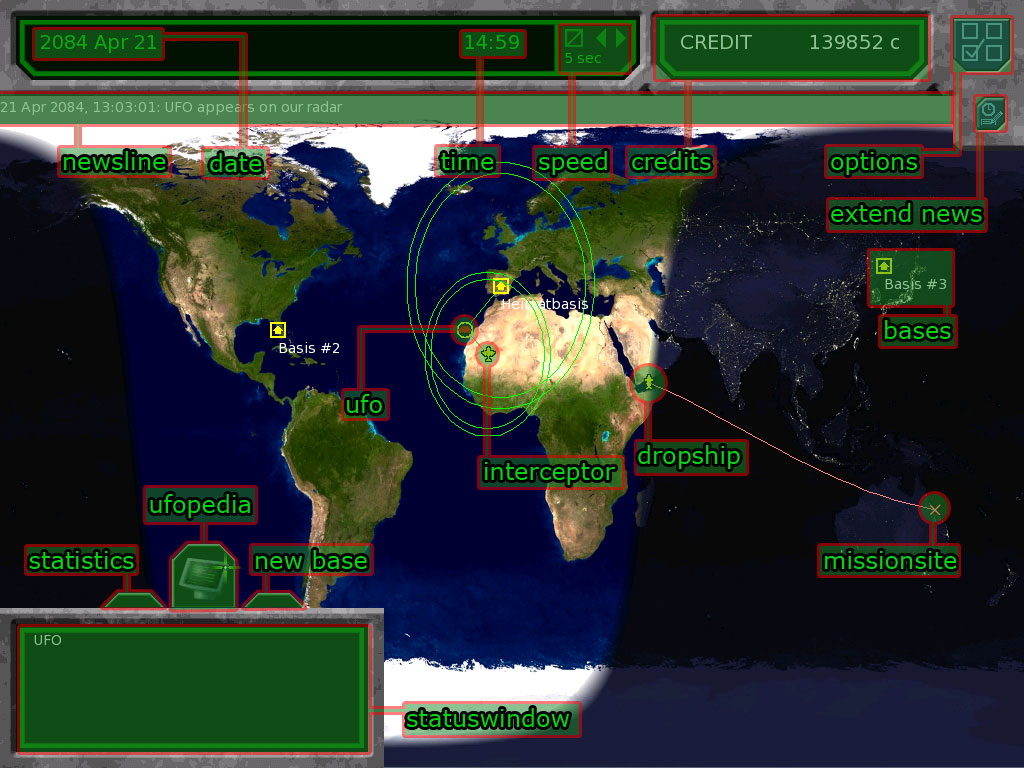
\includegraphics[width=\textwidth]{images/geoscape_final.jpg}

\newpage

\subsubsection{Status Window}
Here some general information(e.g. stats, descriptions) will show up, depending on the context. More detail on each piece of information is given in subsequent sections.
\subsubsection{Statistics}
If you hover over those registers three different buttons will show up. The leftmost leads to some more detailed statistics about your attempt to save the world. In addition to more general information (like missions won/lost etc.) you can also find out about the attitude of all the UN countries paying you. You should be aware that if you fail to protect particular countries from alien invasions (maybe because your infrastructure is not well established in that region) they will cut your resources -- both financial and potential employees.
\subsubsection{Ufopedia}
The middle button is the Ufopedia, a comprehensive collection of useful information about items, technologies, damage types and so on. As your research proceeds Ufopedia grows as well, so make sure you check out the latest information on your enemies every now and then.
\subsubsection{New base}
The rightmost button gives you the chance to establish a new base anywhere on the map, provided it's on land. A new base, once you have built new structures, can give additional radar range, research and production capacities as well as new hangars for your aircraft.  New bases are completely equal to your first in all ways.
\subsubsection{Date}
Gives you the current date, so you know when it's close to pay day. You should also keep an eye on the date, because while you (in principle) have unlimited time to play the game, the aliens get stronger and better equipped as the game proceeds. It is in humanity's best interest if you can catch up with them sooner than later in order to save your beloved homeworld.
\subsubsection{Time and Game Speed}
This is where you can adjust the gamespeed from 5secs (which is in fact pausing the game) all the way through to 1 day steps. Whatever this is set to, while you are in combat time is stopped and it will be all the same when you return from battle.  The game will also automatically pause for certain events like UFO spottings and landings.
\subsubsection{Credits}
Never forget that you can't spend what you don't have.
\subsubsection{Options}
Gets you to the Options-menu where you can load and save your game as well as start a new one.
Through ``exit'' you reach the main menu where you can change game settings and continue your current game (via Single Player $\rightarrow$ Continue)
\subsubsection{News and extended news}
The permanent news line in the upper left always represents the latest news (such as promotions / cashflow / attacks / UFO-sightings) while the extended news button pops up a list of the last 20 new lines. So whenever you notice news, make sure to check the button as well so you don't miss anything. 
\subsubsection{Bases}
The yellow houses represent your bases. Circles around them (popping up later in the game) represent the range of their radars. If you want to ``enter'' a base, just click on its symbol.
\subsubsection{Your dropship}
This is the one that gets your squad to action. Clicking on it once brings up some general data about your ship, like fuel, speed, status and number of assigned soldiers. A second click while it's selected opens a submenu where you may give/change orders, such as sending it back home.
\subsubsection{Your interceptors}
The job of those fast ships is to shoot enemy UFOs down. If your interceptor catches up with a UFA, the dogfight is calculated based on the equipment of both ships; the results are shown on screen. A single click selects the interceptor, while a click on the map will order it to move it there. A second click while the ship is selected brings up a window where you might give it more advanced orders.
\subsubsection{Upcoming missions}
This is where the action waits. Selecting a mission will give you a short description on the status screen while a second one allows you to select a ship to bring in the troops you want.

\section{Your base}
Your bases have to fulfil a wide range of tasks, ranging from researching and producing new equipment, gathering background information on the invaders and supplying the infrastructure to react to any alien incursion. You can change the name of your bases by clicking on the pen-icon right next to its name shown on base screen. You can also cycle through all your current bases using the arrow icons. In the following we will list all relevant screens so you can get familiar with the base management system.

\subsection{Buildings}
This is where you order the construction of additional facilities for your base.  Building laboratories will allow you to increase your research cap, hospitals will allow you to hasten your soldiers' healing.
Before you place a new building, make sure you have read its ufopedia entry. There you can find out if the new site requires additional buildings (for example a power plant) or what it's actually used for. Another important aspect when expanding your base is building time. Buildings vary quite a bit in this regard. Keep in mind that at least a power plant and command centre are needed for most other buildings to be useful. Don't forget, new bases can be built using the world-map, so you don't need to place all facilities in one site. You will want to consider this, as space on individual bases is limited.

\subsection{Aircraft}
This menu brings up a screen where you manage that base's aircraft. This includes not only equipping your vessels with your latest equipment, but also buying new ones or transferring them to another base. You can also circle through all your aircraft using the left and right arrow icons in the window displaying the current aircraft. You can also call a ship back to base or launch it from here, although you're more likely to want to do this from the Geoscape display.

Probably the most important sub-menu here is ``Equip Aircraft''.  This brings up a screen which allows you to choose which soldiers to assign to your selected aircraft. Obviously this is quite important when it comes to your dropship. A standard dropship has room for 8 soldiers, and you will almost always want to use all of them. In order to choose the best soldiers for an upcoming mission you are provided with an picture of your selected character and his / her statistics. A simple click on the `X' or$\surd$ assigns or removes the selected soldier from the current ship. You may also rename your fighters using the ``edit'' button in the upper right, just next to current soldier's name. Also please notice that while you can assign one soldier to an interceptor ship, this is unlikely to do you any good.

Once you have made your decision who to take to battlefield, confirm your selection using the button in the very bottom right corner, which will bring up the inventory screen. You can re-do your troop selection as often as you want, provided the ship in question hasn't left the base.

At the inventory screen, you can equip your soldiers for their upcoming missions. The different sections of this screen should be quite self explanatory; nevertheless we will comment on some of its basic features. In the upper left you see all soldiers assigned to the current aircraft. On the opposite side of the screen, you see the soldier with his / her inventory. The amount of space an item requires is represented by the number of ``squares'' covered. The biggest part of the screen is used by your base's item stock. In order to make it easier to use the rather big amount of items you can choose one of 4 categories (primary/secondary/misc/armor) to be displayed here.  Simple drag \and drop gets any item from bases stock to the specific inventory of your soldiers. Weapons shown with a red background lack the required ammo and aren't useable. You may equip them anyway but unless you get the required ammunition from somewhere else they won't be of any use. In order to assist you in your task to equip every soldier with a weapon he can handle effectively the lower left shows the soldiers statistics (for details on stats please refer to the appendix or ufopedia). Please keep in mind that some weapons utilise two weapon proficiencies depending on the chosen firemode. Alternatively to the soldier's stats window you can change this to an object details view which presents the basic stats (one / two handed, round per clip, firemodes, damage, etc.) of an item. For details on damage and firemodes of a weapon you need to view the details of the according clip / ammunition, as some weapons can be equipped with different types of ammo. A simple click on the arrow symbol in the very bottom right corner confirmes your selections and gets you back to the aircraft screen.

\subsection{Buy / Sell Equipment}
Here you can get new equipment from the global market or get rid of any item you don't have further use for. Please be aware that the items not carried by your soldiers at the end of a mission are sold automatically. Details will be displayed on missions summery screen. If you want to use the items captured you can simply buy them back here. As there is no differences between purchasing and selling prices you won't lose money doing so. This is very likely to be changed once the whole economy thing is set up right till then global market can be exploited as a kind of unlimited equipment storage. Please notice that the amount of any kind of items available may change in the course of the game as your reputation in the world changes. In order to help keeping an overview all items are sorted into four categories again (primary, secondary, misc, armor).

\subsection{Transfer}
Here you can transfer your equipment between different bases.
%moretocome

\subsection{Research}
As research is a critical factor in your attempts to defend earth against the alien threat it is essential to keep your R \and D department busy not only in order to get the lastest weapon technology but to gather background information about your enemy and ways to finally defeat him. The basic features of the research screen are rather simple. While the left part gives all possible research options the right part shows details on the selected subject. In order to discover new research options its usually necessary to capture either at least one kind of the regarding item or a certain key item that offers new information about the alien threat. Sometimes a simple prototype of some alien tech is not enough to get your research started. In such cases the research option is given in grey letters as it requires further research on some other more basic field beforehand. The concrete dependencies for each technology are given in its details shown on the right side of the screen.

To assign a given amount of scientists to a research project just use the left / right arrow-icons next to the technology in question. The left arrow will add scientist to the research while the right one will decrease the amount of scientists working on that project.\\
The actual progress-status is given in the left window. Hint: while it is possible to work on several technologies at the same time in most cases its a better strategy to focus on one research at a time.

\subsection{Production}
Here you can built equipment that is not available on global market or a result of your research departments efforts. To order an item to be build simply select it on the left part of the screen and adjust the amount to be build using the arrow-icons under its image on the right part. Also, please notice that the production cost is taken from your cash when one item is started. For example while: 3 assault rifles cost 63000 you need only 21000 to start production.

\subsection{Hire employees}
Using this screen you can add further personal to your organisation. While especially in the beginning people do not trust in your ability to counter the aliens they might be more enthusiastic (and therefore willing to work for you) as you proceed in the game. On the left side you find all members of one group (soldiers/medics/workers/scientist) listed. clicking on the `X' or $\surd$ hires or fires them. You can discard / select them as often as you want, they will never get angry at you. But please be aware that personnel you hire in one base won't be accessible from another base. So if you want to fire someone make sure you are in the corresponding base. Also you should keep in mind that the amount of personnel that can work in your base might be limited by the base's housing or working facilities. AFAIK this is not the case right now. also it doesn't seem possible to hire more than 19 persons of one group for the simple reason that there is no way to scroll down the list.

\section{Gamemechanics / Management}
%maybe to be extended significantly
\subsection{Research}
Every unknown alien technology must be researched by your scientists. You will get a brief description for each technology in your mail client - make sure you read it.
% extend this

\subsection{Promotions}
While the actual implementation is still under heavy discussion a few comments might help to understand how it works now. Different you ones first thought the main criteria for promotions is not the missions / kills ratio but the mind skill. You simply don't want an psychopathic, thrill seeking terminator like guy as squadleader but someone who is mentally stable ;) Also, up to now, there is only one member of you squad that is going to be promoted while the rest is left with nothing.
Here a list of the different badges and their corresponding ranks.

\subsection{Interceptions}
%todo

\subsection{UFO-Recoveries}
%todo

\subsection{Alien autopsies}
%todo

\begin{tabular}{ccc}

\includegraphics[scale=1]{images/badges_rekrut_final.jpg} & 
\includegraphics[scale=1]{images/badges_sergeant_final.jpg} & 
\includegraphics[scale=1]{images/badges_hauptmann_final.jpg}\\
Private & Sergeant & Hauptmann\\
\end{tabular} 
